%! Author = leocr
%! Date = 04/01/2025

% Preamble
\documentclass[12pt]{article}

% Packages
\usepackage[top=1in, bottom=1.2in, left=1in, right=1in]{geometry}
\usepackage{amsmath}
\usepackage{upgreek}
\usepackage{graphicx}
\usepackage{subcaption}
\usepackage{hyperref}
\setlength{\parindent}{0pt}



% Document
\begin{document}
    \section{Introduction}
    The aim of this work is to estimate the parameters of the SIR model.
    In particular, I will focus on the first wave of contagion of the Coronavirus pandemic in Italy.

    \begin{figure}[h!]
        \label{fig:covid_italy}
        \centering
        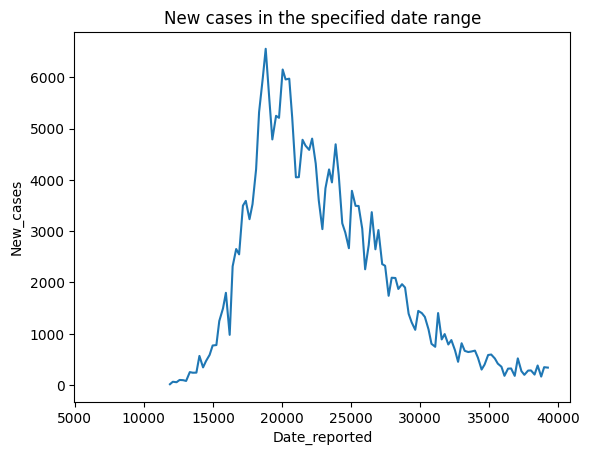
\includegraphics[width=.8\linewidth]{plots/real_data}
        \caption{New infections per day in Italy}
    \end{figure}

    \section{Model}

    \subsection{Standard SIR model}
    My first try was with the following differential equation for the total infected population:

    $$\frac{dN}{dt} = r N \left(1-\frac{N}{K}\right), \quad N(0)=N_0$$

    Which admits the following solution:

    $$N(t) = \frac{K}{1+ \left(\frac{K-N_0}{N_0}\right) e^{-rt}}$$

    That has a flex (i.e. the max of the new infections curve) in:
    $$ t^* = \frac{1}{r}\ln \left(\frac{K-N_0}{N_0}\right)$$

    To use a linear regression, the differential equation can be discretized into:
    $$ N_{t+1} = \alpha_1 N_t + \alpha_2 N_{t}^2$$

    So the parameter can be found using:
    $$ r = \alpha_1-1, \quad K= \frac{1-\alpha_1}{\alpha_2}$$

    \subsection{Bernoulli equation model}

    However, the solution of the SIR model yields a symmetric curve, therefore a more appropriate model that can deliver the right-hand skewness of the contagion curve is:
    \begin{equation}
        N_{t+1} = \alpha_1 N_t + \alpha_2 N_{t}^{1 + \varepsilon},
        \label{eq:equation0}
    \end{equation}
    with $\varepsilon \in (0,1)$

    Using Bernoulli transformation:
    $$V = N^{-\varepsilon}, \qquad \frac{\dot V}{V} = -r \varepsilon \frac{\dot N}{N}, \quad \Rightarrow \quad \dot V = -r\varepsilon V + \frac{r\varepsilon}{K}. $$

    Which has close form solution:
    $$ V(t) = K^{-1} + \left(V_0-K^{-1}\right)e^{-r\varepsilon t} \quad \Rightarrow \quad N(t)=\frac{1}{\left(K^{-1} + \left(N_0^{-\varepsilon}-K^{-1}\right)e^{-r\varepsilon t}\right)^\varepsilon}\,.$$

    The peak of the new cases is determined by solving:
    $$ \ddot N = -\frac{V^{-\frac{1+\varepsilon}{\varepsilon}}}{\varepsilon} \left(\ddot V -\frac{1+\varepsilon}{\varepsilon} \frac{\dot V ^2}{V}\right) \quad \to \quad t^* = \frac{1}{\varepsilon r}\ln \left(\varepsilon K N_0^{-\varepsilon}-\varepsilon\right) $$

    Where:
    $$ \dot V = -r\varepsilon\left(V_0-K^{-1}\right)e^{-r\varepsilon t}, \qquad \ddot V = (r\varepsilon)^2 \left(V_0-K^{-1}\right)e^{-r\varepsilon t}. $$

    In terms of finite differences:
    $$ V_{t+1} = \beta_0 + \beta_1 V_t,$$

    where:
    $$\beta_0 = -\alpha_2\varepsilon = \frac{r \varepsilon}{K}, \quad \beta_1=\varepsilon(1-\alpha_1) = - r\varepsilon.$$

    \newpage

    \section{Estimation}\label{sec:estimation}
    \subsection{Preliminary Regression}
    Let's regress the following model with OLS:
    \begin{equation}
        V_{t+1} = \beta_0 + \beta_1 V_t + U_t,
    \end{equation}
    where $V_t=N_t^{-\varepsilon}$, for given values of $\varepsilon$.
    I tried with the following values: $\varepsilon \in \{1, 0.1, 0.01, 0.001, 0.0001\}$.
    The OLS regression yielded the following results:

    \begin{table}[h!]
\label{tab:preliminary-regression}
\centering
    \begin{tabular}{llllll}
    \hline
                   & \varepsilon =: 1.0 & \varepsilon =: 0.1 & \varepsilon =: 0.01 & \varepsilon =: 0.001 & \varepsilon =: 0.0001  \\
    \hline
    $\beta_0$      & 0.0000*            & 0.0211***          & 0.0501***           & 0.0547***            & 0.0552***              \\
                   & (0.0000)           & (0.0006)           & (0.0013)            & (0.0014)             & (0.0014)               \\
    $\beta_1$      & 0.6348***          & 0.9278***          & 0.9433***           & 0.9446***            & 0.9447***              \\
                   & (0.0071)           & (0.0019)           & (0.0014)            & (0.0014)             & (0.0014)               \\
    \hline
    R-squared      & 0.9827             & 0.9994             & 0.9997              & 0.9997               & 0.9997                 \\
    R-squared Adj. & 0.9826             & 0.9994             & 0.9997              & 0.9997               & 0.9997                 \\
    N              & 142                & 142                & 142                 & 142                  & 142                    \\
    \hline
    \end{tabular}
    \caption{Standard errors in parentheses. \newline
$* p<0.1$, $** p<0.05$, $***p<0.01$}
\end{table}
\bigskip


    Overall, the assumption of a linear relationship between $V_t$ and $V_{t-1}$ seems to hold, as long as $\varepsilon$ is small enough.


    \begin{figure}[h!]
        \centering
        \begin{subfigure}[b]{0.3\textwidth}
            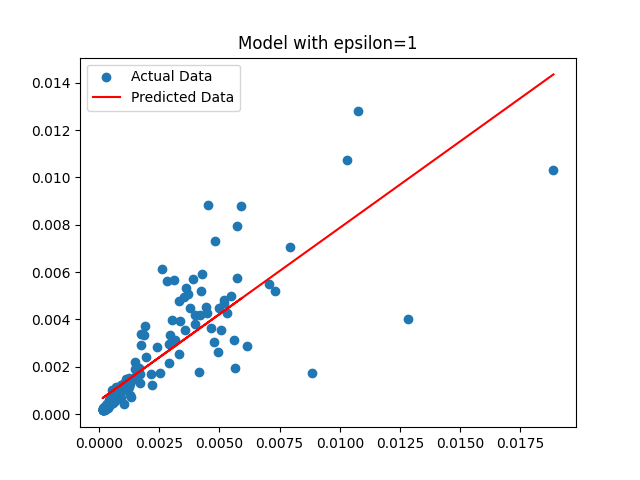
\includegraphics[width=.9\linewidth]{plots/epsilon_1}
            \caption{$\varepsilon = 1$}
        \end{subfigure} \quad
        \begin{subfigure}[b]{0.3\textwidth}
            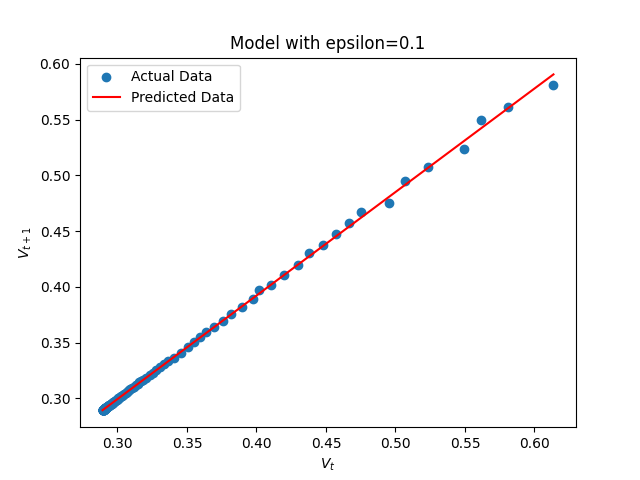
\includegraphics[width=.9\linewidth]{plots/epsilon_0.1}
            \caption{$\varepsilon = 0.1$}
        \end{subfigure} \quad
        \begin{subfigure}[b]{0.3\textwidth}
            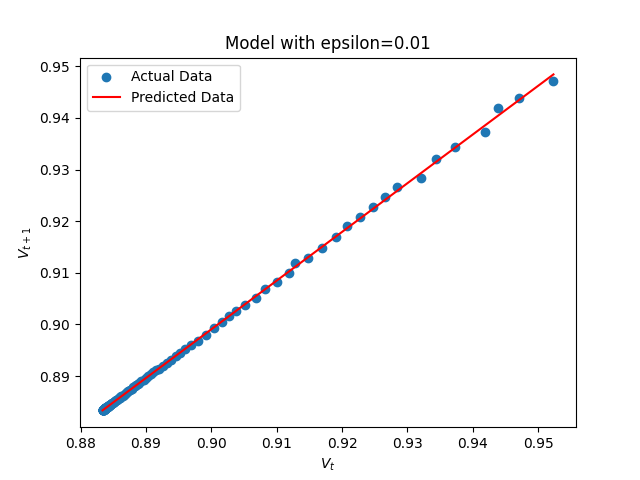
\includegraphics[width=.9\linewidth]{plots/epsilon_0.01}
            \caption{$\varepsilon = 0.01$}
        \end{subfigure}\\
        \begin{subfigure}[b]{0.3\textwidth}
            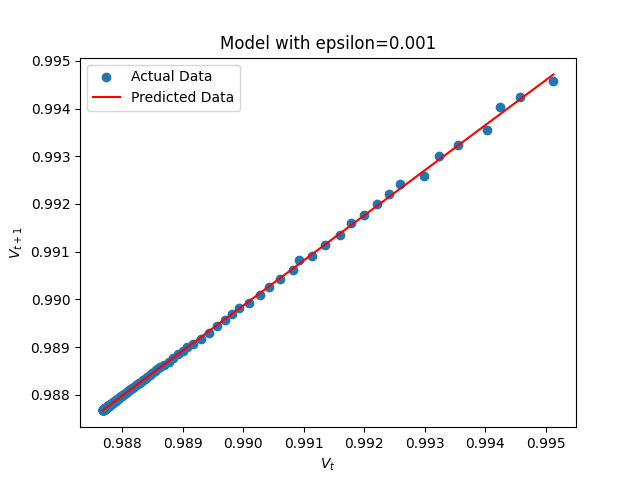
\includegraphics[width=.9\linewidth]{plots/epsilon_0.001}
            \caption{$\varepsilon = 0.001$}
        \end{subfigure} \quad
        \begin{subfigure}[b]{0.3\textwidth}
            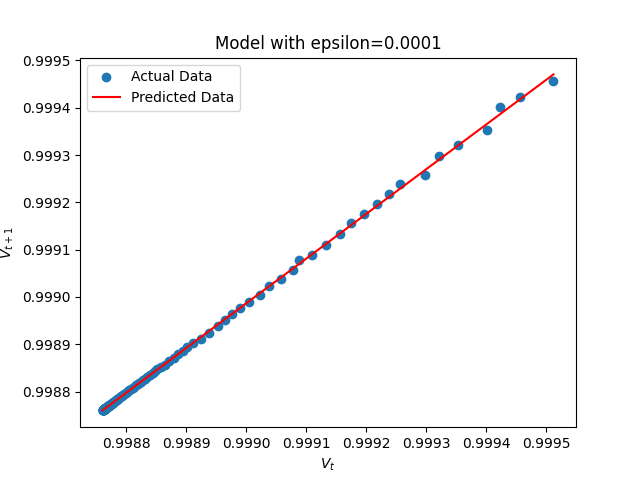
\includegraphics[width=.9\linewidth]{plots/epsilon_0.0001}
            \caption{$\varepsilon = 0.0001$}
        \end{subfigure}
        \caption{Regression Plot $V_t$ over $V_{t-1}$}
        \label{fig:vt_vs_vt1}
    \end{figure}

\newpage


    \subsection{Ramsey Test}

    Assuming $\varepsilon \simeq 0$, we can expand $N_{t}^{\,1+\varepsilon}$ as:
    \begin{equation}
        N_{t}^{\,1+\varepsilon} \simeq N_{t} \left( 1 + \varepsilon \ln N_{t} + \frac{\varepsilon^2 (\ln N_{t})^2}{2} + \frac{\varepsilon^3 (\ln N_{t})^3}{6} \right).
    \end{equation}

    So:
        \begin{equation}
        N_{t+1} = (\alpha_1 + \alpha_2) N_{t} + \varepsilon \alpha_2 N_{t}\ln N_{t} + \varepsilon^2 \alpha_2 N_{t} \frac{ (\ln N_{t})^2}{2} + \varepsilon^3 \alpha_2 N_{t} \frac{(\ln N_{t})^3}{6}.
        \end{equation}

    So by regressing on the nonlinear terms:

    \begin{table}[htbp]\centering
\def\sym#1{\ifmmode^{#1}\else\(^{#1}\)\fi}
\caption{Ramsey Test}
\begin{tabular}{l*{1}{c}}
\hline\hline
                    &\multicolumn{1}{c}{(1)}\\
                    &\multicolumn{1}{c}{Y}\\
\hline
X                   &      -3.953         \\
                    &     (-1.00)         \\
[1em]
hat\_Y\_ln\_hat\_Y      &       1.606         \\
                    &      (1.62)         \\
[1em]
hat\_Y\_ln\_hat\_Y2     &      -0.158         \\
                    &     (-1.90)         \\
[1em]
hat\_Y\_ln\_hat\_Y3     &     0.00493\sym{*}  \\
                    &      (2.12)         \\
[1em]
Constant            &    -13649.1         \\
                    &     (-1.39)         \\
\hline
Observations        &         151         \\
\hline\hline
\multicolumn{2}{l}{\footnotesize \textit{t} statistics in parentheses}\\
\multicolumn{2}{l}{\footnotesize \sym{*} \(p<0.05\), \sym{**} \(p<0.01\), \sym{***} \(p<0.001\)}\\
\end{tabular}
\end{table}


    I can then reasonably assume there is some nonlinearity at play in the relationship between $N_{t-1}$ and $N_t$.
    \begin{figure}[h!]
            \centering
            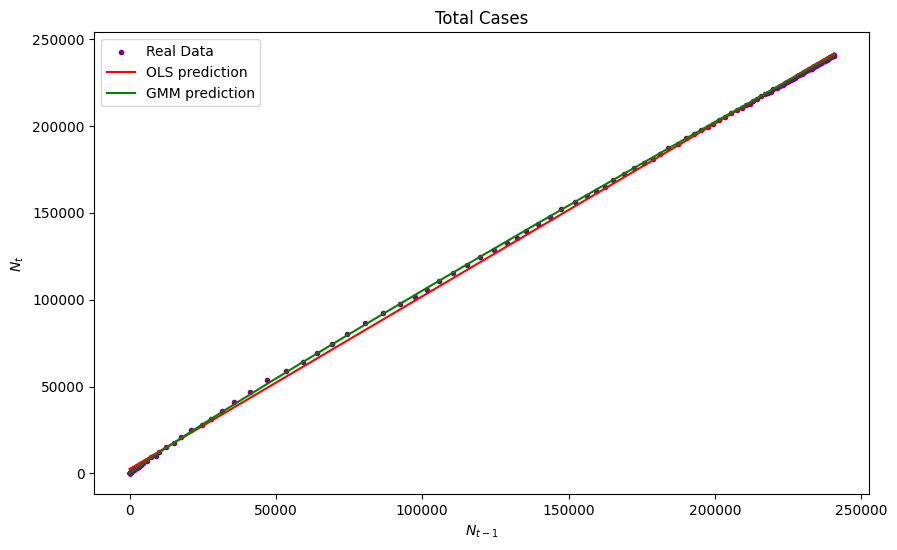
\includegraphics[width=0.6\linewidth]{plots/regression_comparison_1}\quad
            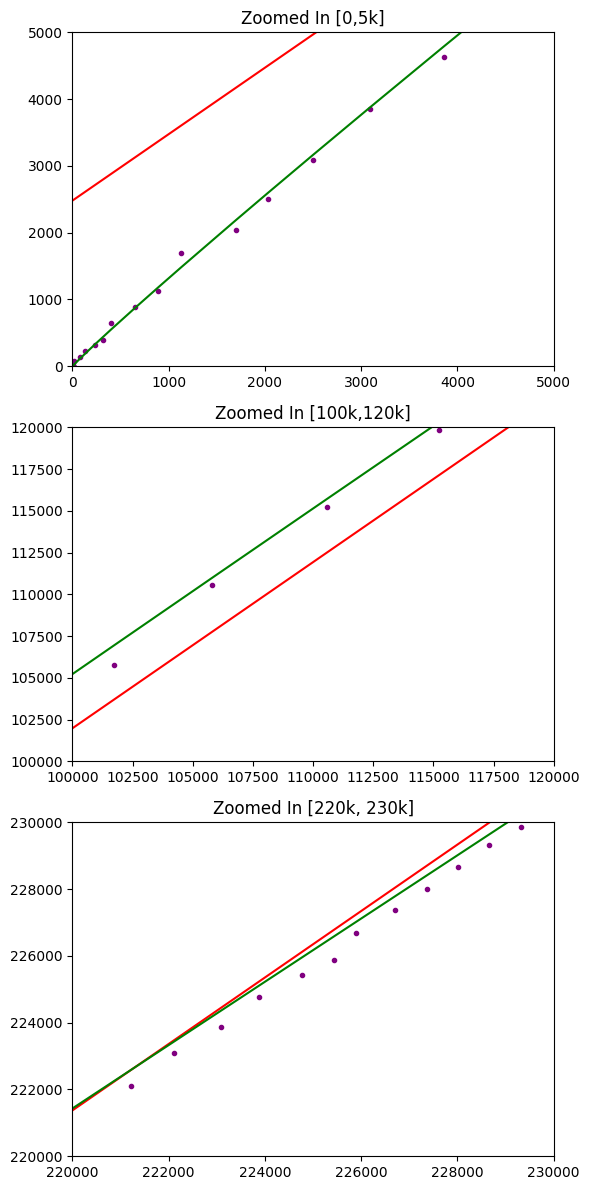
\includegraphics[width=0.2\linewidth]{plots/regression_comparison_2}
            \caption{$N_t$ vs $N_{t-1}$ comparison between OLS and G2 model}
            \label{fig:plot_gmm_ols_comp}
        \end{figure}


\subsection{GMM estimation with Stata}

    Let's consider the model:
    \begin{equation}
        N_{t} = \alpha_1 N_{t-1} + \alpha_2 N_{t-1}^{1 + \varepsilon} + U_t
        \label{eq:equation1}
    \end{equation}

    I assume that $U_t$ is mean independent of all the $N_s$ for $s\leq t-1$.
    For 3 parameters, at least 3 instruments are needed.
    The following set of instruments were tried:
    \begin{table}[h!]
        \centering
        \begin{tabular}{l c}
            Model & Instruments \\ \hline
            S3 & $N_{t-1}, N_{t-2}, N_{t-3}$ \\
            S4 &  $N_{t-1}, N_{t-2}, N_{t-3}, N_{t-4}$ \\
            Sln &  $N_{t-1}, N_{t-2}, N_{t-3}, N_{t-1} \ln N_{t-1}$
        \end{tabular}
        \label{tab:models_stat}
    \end{table}

    The results are as follows:
    \begin{table}[htbp]\centering
\newcommand{\sym}[1]{\ifmmode^{#1}\else\(^{#1}\)\fi}
\caption{GMM Regression Table}
\begin{tabular}{l*{4}{c}}
\hline\hline
Instruments           &\multicolumn{1}{c}{$N_1$ $N_2$}&\multicolumn{1}{c}{$N_1$ $N_2$ $N_3$}&\multicolumn{1}{c}{$N_1$ $N_2$ $N_3$ $N_4$}&\multicolumn{1}{c}{$N_1$ $N_2$ $N_3$ $N_1\ln N_1$}\\
\hline
$\alpha_1$           &       4.280         &       7.049         &       7.457         &       7.503         \\
                    &     (6.681)         &         (.)         &         (.)         &         (.)         \\
\hline
$\alpha_2$           &      -2.528         &      -4.981\sym{***}&      -5.466\sym{***}&      -5.474\sym{***}\\
                    &     (6.514)         &    (0.0550)         &    (0.0453)         &    (0.0493)         \\
\hline
$\varepsilon$       &      0.0210         &      0.0157\sym{***}&      0.0135\sym{***}&      0.0140\sym{***}\\
                    &    (0.0436)         &  (0.000896)         &  (0.000672)         &  (0.000730)         \\
\hline
J                   &                     & 252496718.1         & 161236752.4         & 209017433.8         \\
J\_df                &           0         &           2         &           3         &           3         \\
rank                &           3         &           2         &           2         &           2         \\
\hline\hline
\multicolumn{5}{l}{\footnotesize Standard errors in parentheses}\\
\multicolumn{5}{l}{\footnotesize \sym{*} \(p<0.05\), \sym{**} \(p<0.01\), \sym{***} \(p<0.001\)}\\
\end{tabular}\label{tab:gmm_table}
\end{table}


    All the model failed to converge in Stata (tried with different criteria, but without luck).
    \begin{figure}[h!]
        \centering
        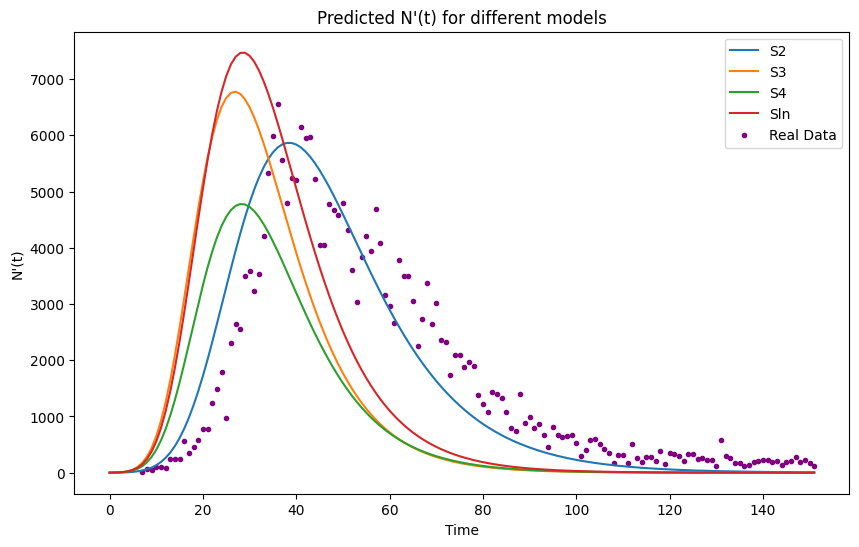
\includegraphics[width=0.8\linewidth]{plots/gmm_stata}
        \caption{Comparison between real data and the predicted new cases using the parameters from Stata.}
        \label{fig:plot_gmm_stata}
    \end{figure}

\newpage

\subsection{GMM estimation with grid search}

    I therefore implemented the GMM in python, with the minimization done by grid search on the parameters.
    The following set of instruments were tried:

    \begin{table}[h!]
        \centering
        \begin{tabular}{l c}
            Model & Instruments \\ \hline
            G3 & $N_{t-1}, N_{t-2}, N_{t-3}$ \\
            G4 & $N_{t-1}, N_{t-2}, N_{t-3}, N_{t-4}$ \\
            G5 & $N_{t-1}, N_{t-2}, N_{t-3}, N_{t-4}, N_{t-5}$
        \end{tabular}
        \label{tab:models_grid_search}
    \end{table}

    The results are as follows:
    \begin{table}[h!]\centering
%\renewcommand{\sym}[1]{\ifmmode^{#1}\else\(^{#1}\)\fi}
\caption{GMM results using grid search}
\begin{tabular}{l*{3}{c}}
\hline\hline
Model           &\multicolumn{1}{c}{G3}&\multicolumn{1}{c}{G4}&\multicolumn{1}{c}{G5}\\
\hline
$\alpha_1$           &       3.273       &       3.545         &       3.545         \\
                &     (3.919)       &     (5.548)         &     (5.547)         \\
\hline
$\alpha_2$           &      -1.636       &      -1.924         &      -1.924        \\
                &    (3.765)        &    (5.381)         &    (5.381)         \\
\hline
$\varepsilon$             &      0.0265       &      0.0226        &      0.0226         \\
                &  (0.0465)         &  (0.0498)         &  (0.0498)         \\
\hline
J-stat          &                   &  14.5866          &  14.7678 \\
OverId          &       0           &           1         &           2         \\
Samples         &       151         &           151         &           151         \\
\hline\hline
\multicolumn{5}{l}{\footnotesize Standard errors in parentheses}\\
%\multicolumn{5}{l}{\footnotesize \sym{*} \(p<0.05\), \sym{**} \(p<0.01\), \sym{***} \(p<0.001\)}\\
\end{tabular}\label{tab:gmm_table}
\end{table}


    \begin{figure}[h!]
        \centering
        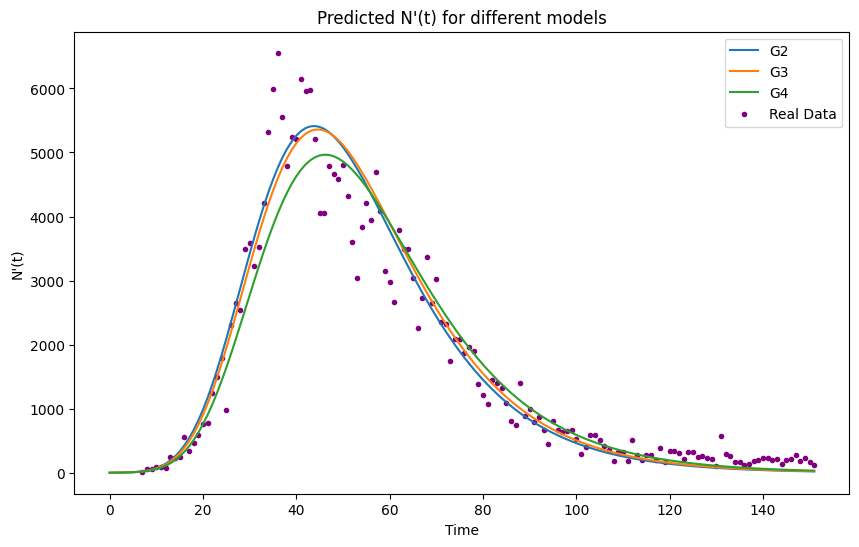
\includegraphics[width=0.8\linewidth]{plots/gmm_grid_search}
        \caption{Comparison between real data and the predicted new cases using the parameters found with the grid search minimization.}
        \label{fig:plot_gmm_grid_search}
    \end{figure}

    \newpage
    \subsection{Specification Test}
    I tested the specifications of model G4 and the validity of instruments $N_{t-4}, N_{t-5}$:
    \begin{itemize}
        \item Hansen test for G4 model specification:
            \begin{equation}
                \hat J_3 = 14.58 > 5.99 =Q_{\chi^2_2}(0.95)
            \end{equation}
            The test rejects the hypothesis of valid specifications, suggesting the model is not well-defined.
        \item EHS test for exogeneity of $N_{t-4}, N_{t-5}$:
            \begin{equation}
                \hat J_5 - \hat J_3 = 1.68 < 5.99 =Q_{\chi^2_2}(0.95)
            \end{equation}
            The test does not reject the validity of instruments $N_{t-4}, N_{t-5}$.
    \end{itemize}
    There are possibly some issues (i.e.\ collinearity of the instruments that hinder the over-identification degrees).

    \subsection{IV model}
    To solve the issue of possible collinearity, I introduced the following instruments:
    \begin{itemize}
        \item Daily temperature data (temperature 2m above ground, in Celsius)
        \item Daily mobility data (percent change from baseline of occupation of retail and recreation and transit stations)
    \end{itemize}

    The results are as follows:

    \section{Approximated model}



    \section{Data Sources}
    \begin{itemize}
        \item Covid infection data is available on the Covid section of the WHO website \url{https://data.who.int/dashboards/covid19/}
        \item Temperature data is available on the EU Copernicus Climate Data Store website \url{https://cds.climate.copernicus.eu/}
        \item Mobility data is available on the Google Covid19 Mobility Report website \url{https://www.google.com/covid19/mobility/}
    \end{itemize}








\end{document}